\documentclass[12pt]{article}
\usepackage[margin=0.5in]{geometry}
\usepackage{tikz}
\usepackage{amsmath}
\usepackage{pgfplots}
\usepackage{gensymb}

\begin{document}

\begin{center}
\textbf{11+ Mathematics Mock Exam - Year 4}
\end{center}

\section*{Section 1: Arithmetic}
\begin{enumerate}
  \item Calculate the sum of $43$ and $57$.
  \item Subtract $36$ from $84$.
  \item Multiply $8$ by $5$.
\end{enumerate}

\section*{Section 2: Number and Place Value}
\begin{enumerate}
  \item Write the place value of the digit $7$ in the number $437$.
  \item What is the successor of $99$?
  \item Write the number $1,245$ in words.
\end{enumerate}

\section*{Section 3: Fractions}
\begin{enumerate}
  \item Simplify the fraction $\frac{6}{12}$.
  \item Convert $\frac{3}{5}$ to a decimal.
  \item Add $\frac{2}{3}$ and $\frac{1}{4}$.
\end{enumerate}

\section*{Section 4: Decimals}
\begin{enumerate}
  \item Write $0.85$ as a fraction in simplest form.
  \item Round $2.987$ to the nearest tenth.
  \item Calculate $4.3 \times 2.5$.
\end{enumerate}

\section*{Section 5: Percentages}
\begin{enumerate}
  \item Express $25\%$ as a fraction.
  \item Find $20\%$ of $180$.
  \item Increase $80$ by $15\%$.
\end{enumerate}

\section*{Section 6: Measurement and Geometry}
\begin{enumerate}
  \item Convert $2$ meters to centimeters.
  \item Calculate the perimeter of a rectangle with sides of length $7$ cm and $9$ cm.
  \item Find the area of a triangle with base $6$ cm and height $4$ cm.
\end{enumerate}

\section*{Section 7: Graphs and Bar Charts}
\begin{enumerate}
  \item Use the bar chart below to answer the question: How many students prefer apples?
  
  \begin{center}
  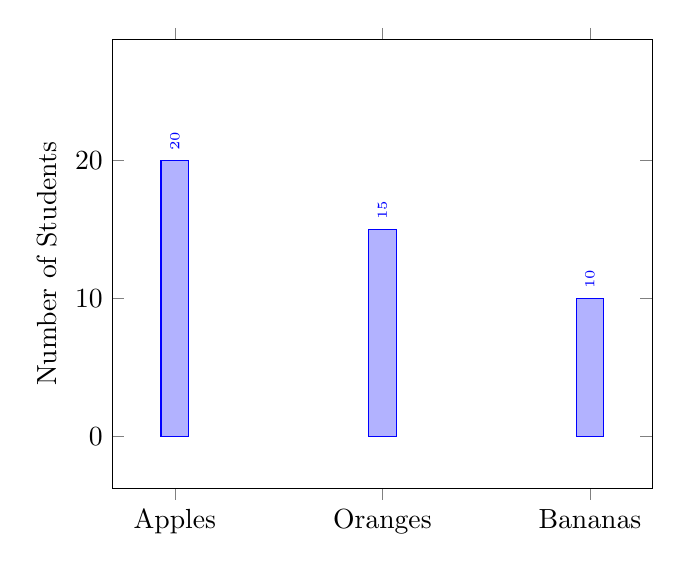
\begin{tikzpicture}
    \begin{axis}[
        ybar,
        ymin=0,
        ymax=25,
        symbolic x coords={Apples, Oranges, Bananas},
        xtick=data,
        ylabel=Number of Students,
        enlargelimits=0.15,
        legend style={at={(0.5,-0.15)},
        anchor=north,legend columns=-1},
        nodes near coords,
        every node near coord/.append style={
            rotate=90,
            anchor=west,
            font=\tiny
        }
    ]
    \addplot coordinates {(Apples,20) (Oranges,15) (Bananas,10)};
    \end{axis}
  \end{tikzpicture}
  \end{center}
  
  \item Which graph represents the temperature throughout a day: a straight line or a curve?
  \item The table below shows the distances traveled by a car over four days. Use the table to answer the question: How many more kilometers did the car travel on Day 3 compared to Day 1?
  
  \begin{center}
  \begin{tabular}{|c|c|}
    \hline
    \textbf{Day} & \textbf{Distance (km)} \\
    \hline
    1 & 35 \\
    2 & 40 \\
    3 & 45 \\
    4 & 30 \\
    \hline
  \end{tabular}
  \end{center}
\end{enumerate}

\end{document}
